\begin{frame}{Grafos Planares}
    \centering\Large
    Um grafo é \textbf{\emph{planar}} se ele pode ser desenhado no plano Euclidiano sem cruzamentos de arestas.
    \bigbreak
    
    \begin{columns}
        \column{0.5\textwidth}
        \begin{figure}
            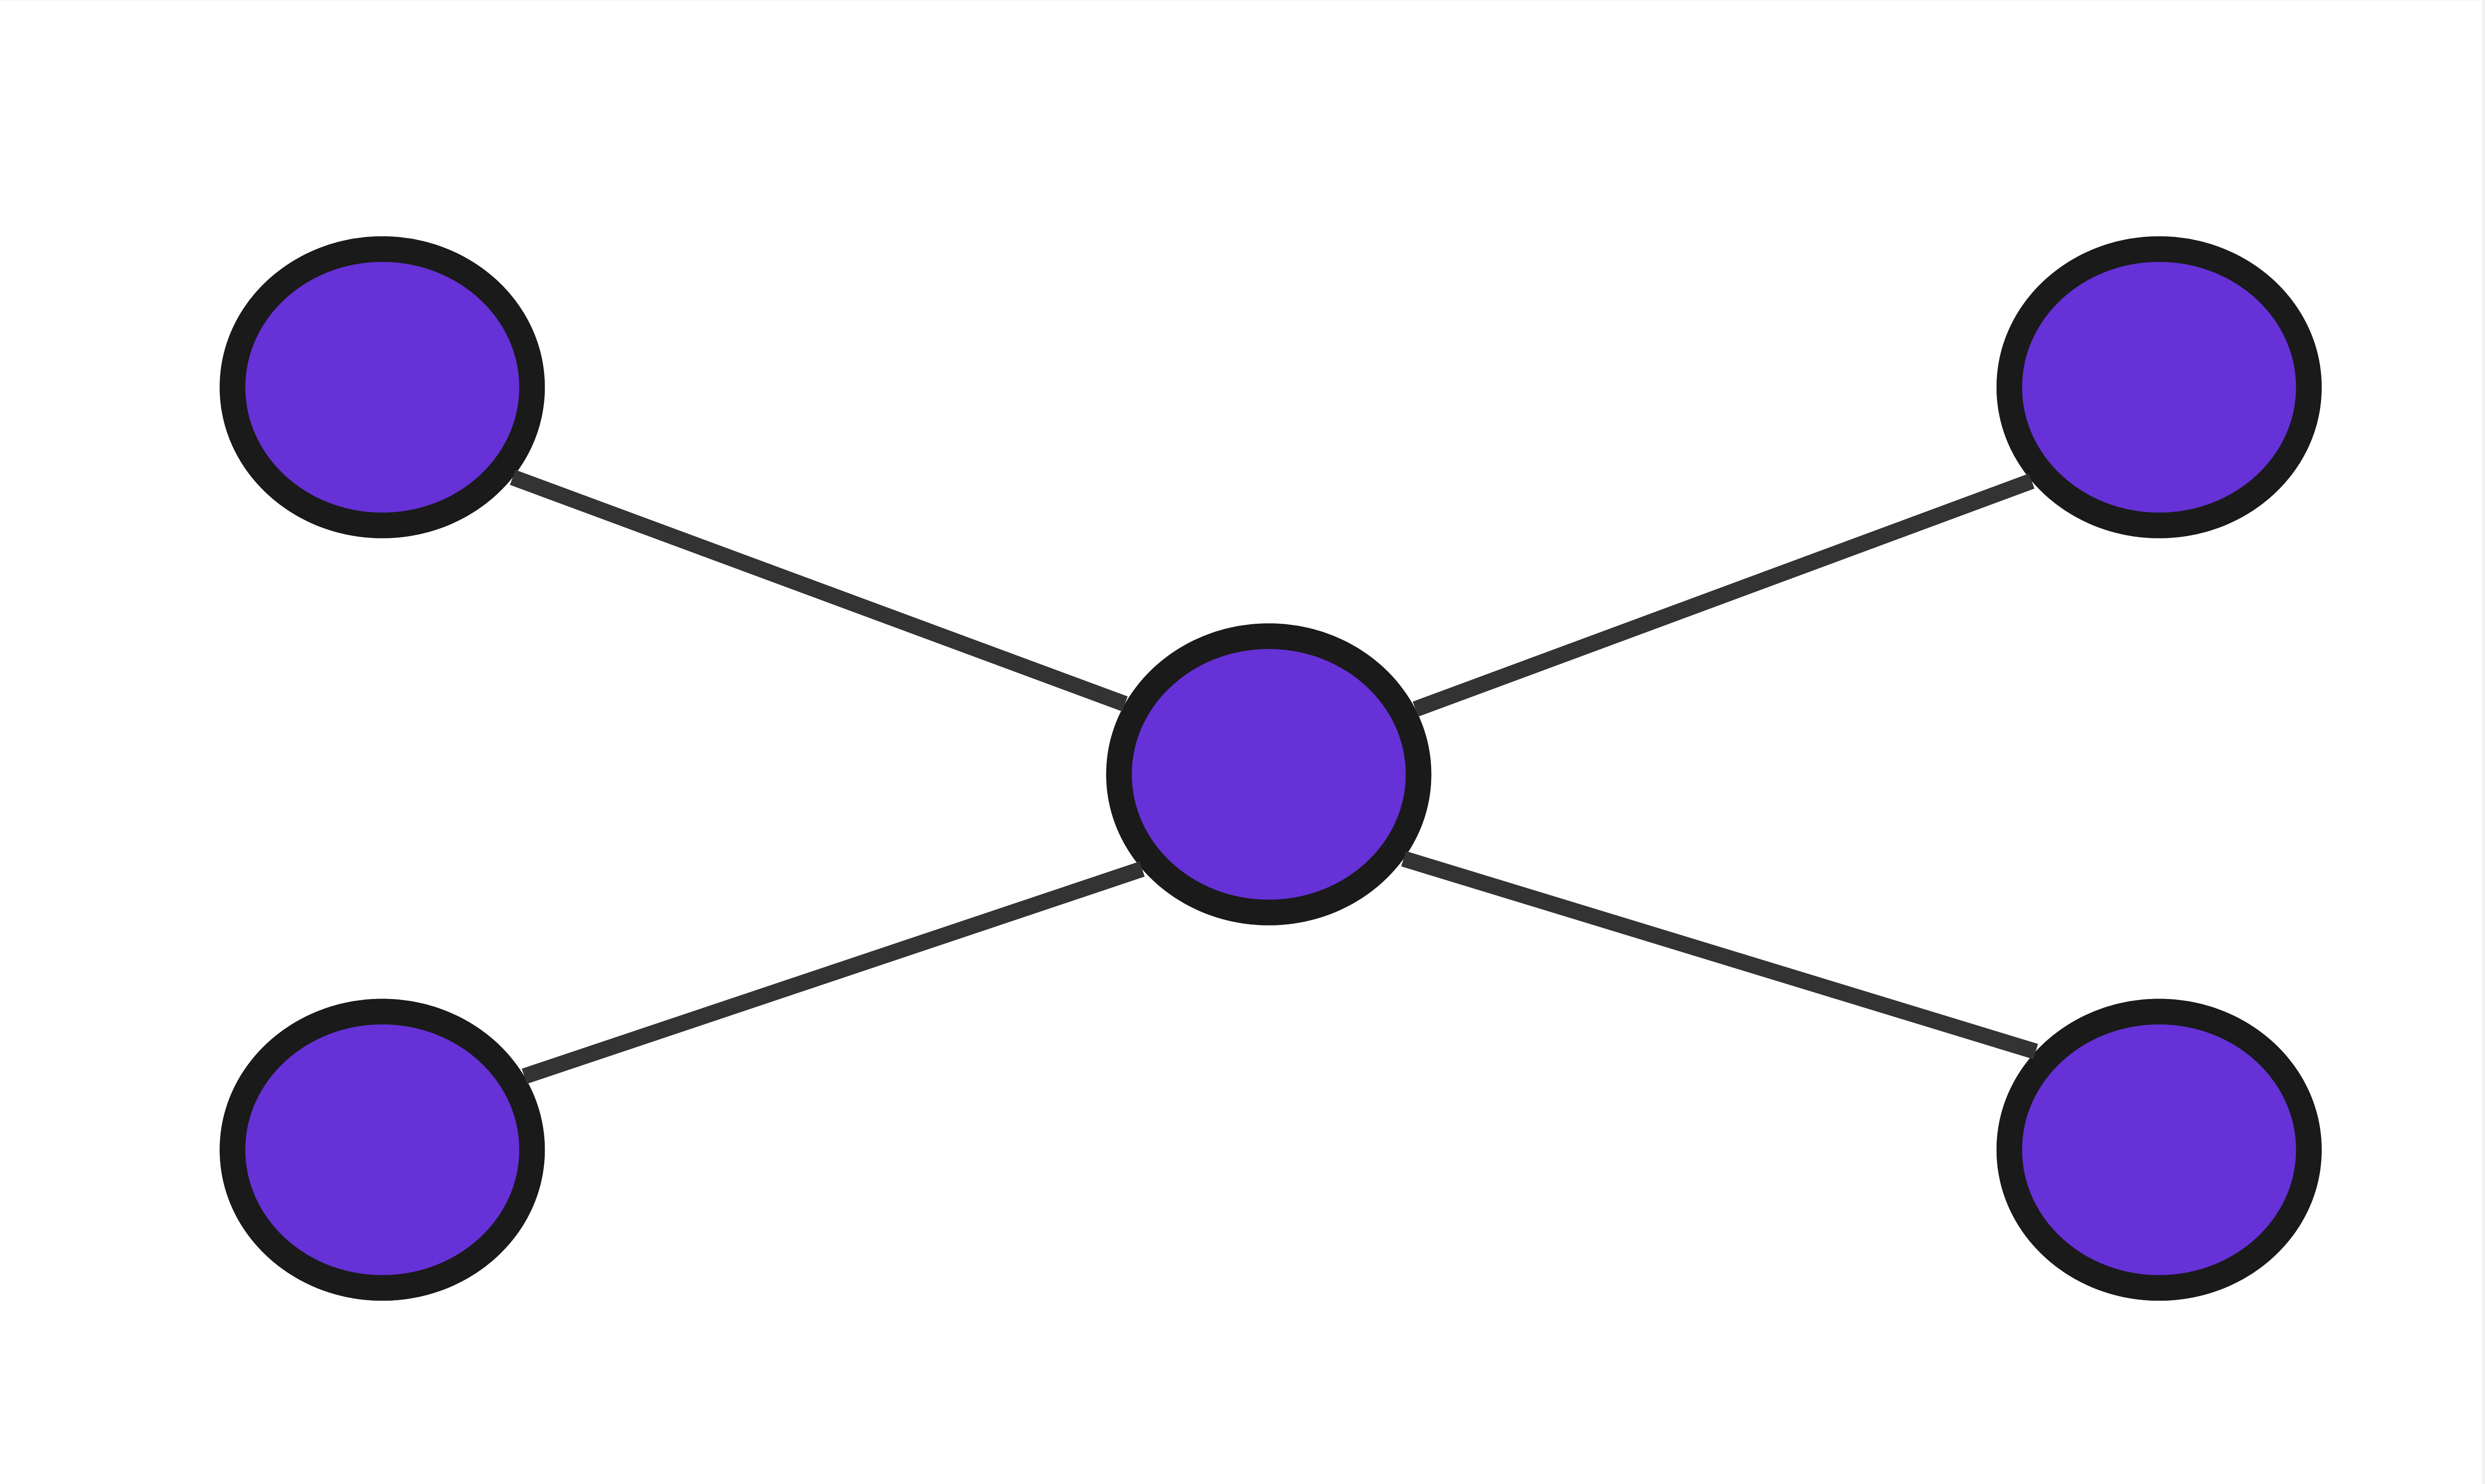
\includegraphics[width=0.9\linewidth]{images/butterfly_graph.jpg}
            \caption*{\textit{Grafo Borboleta}}
        \end{figure}
    
        \column{0.5\textwidth}
        \begin{figure}
            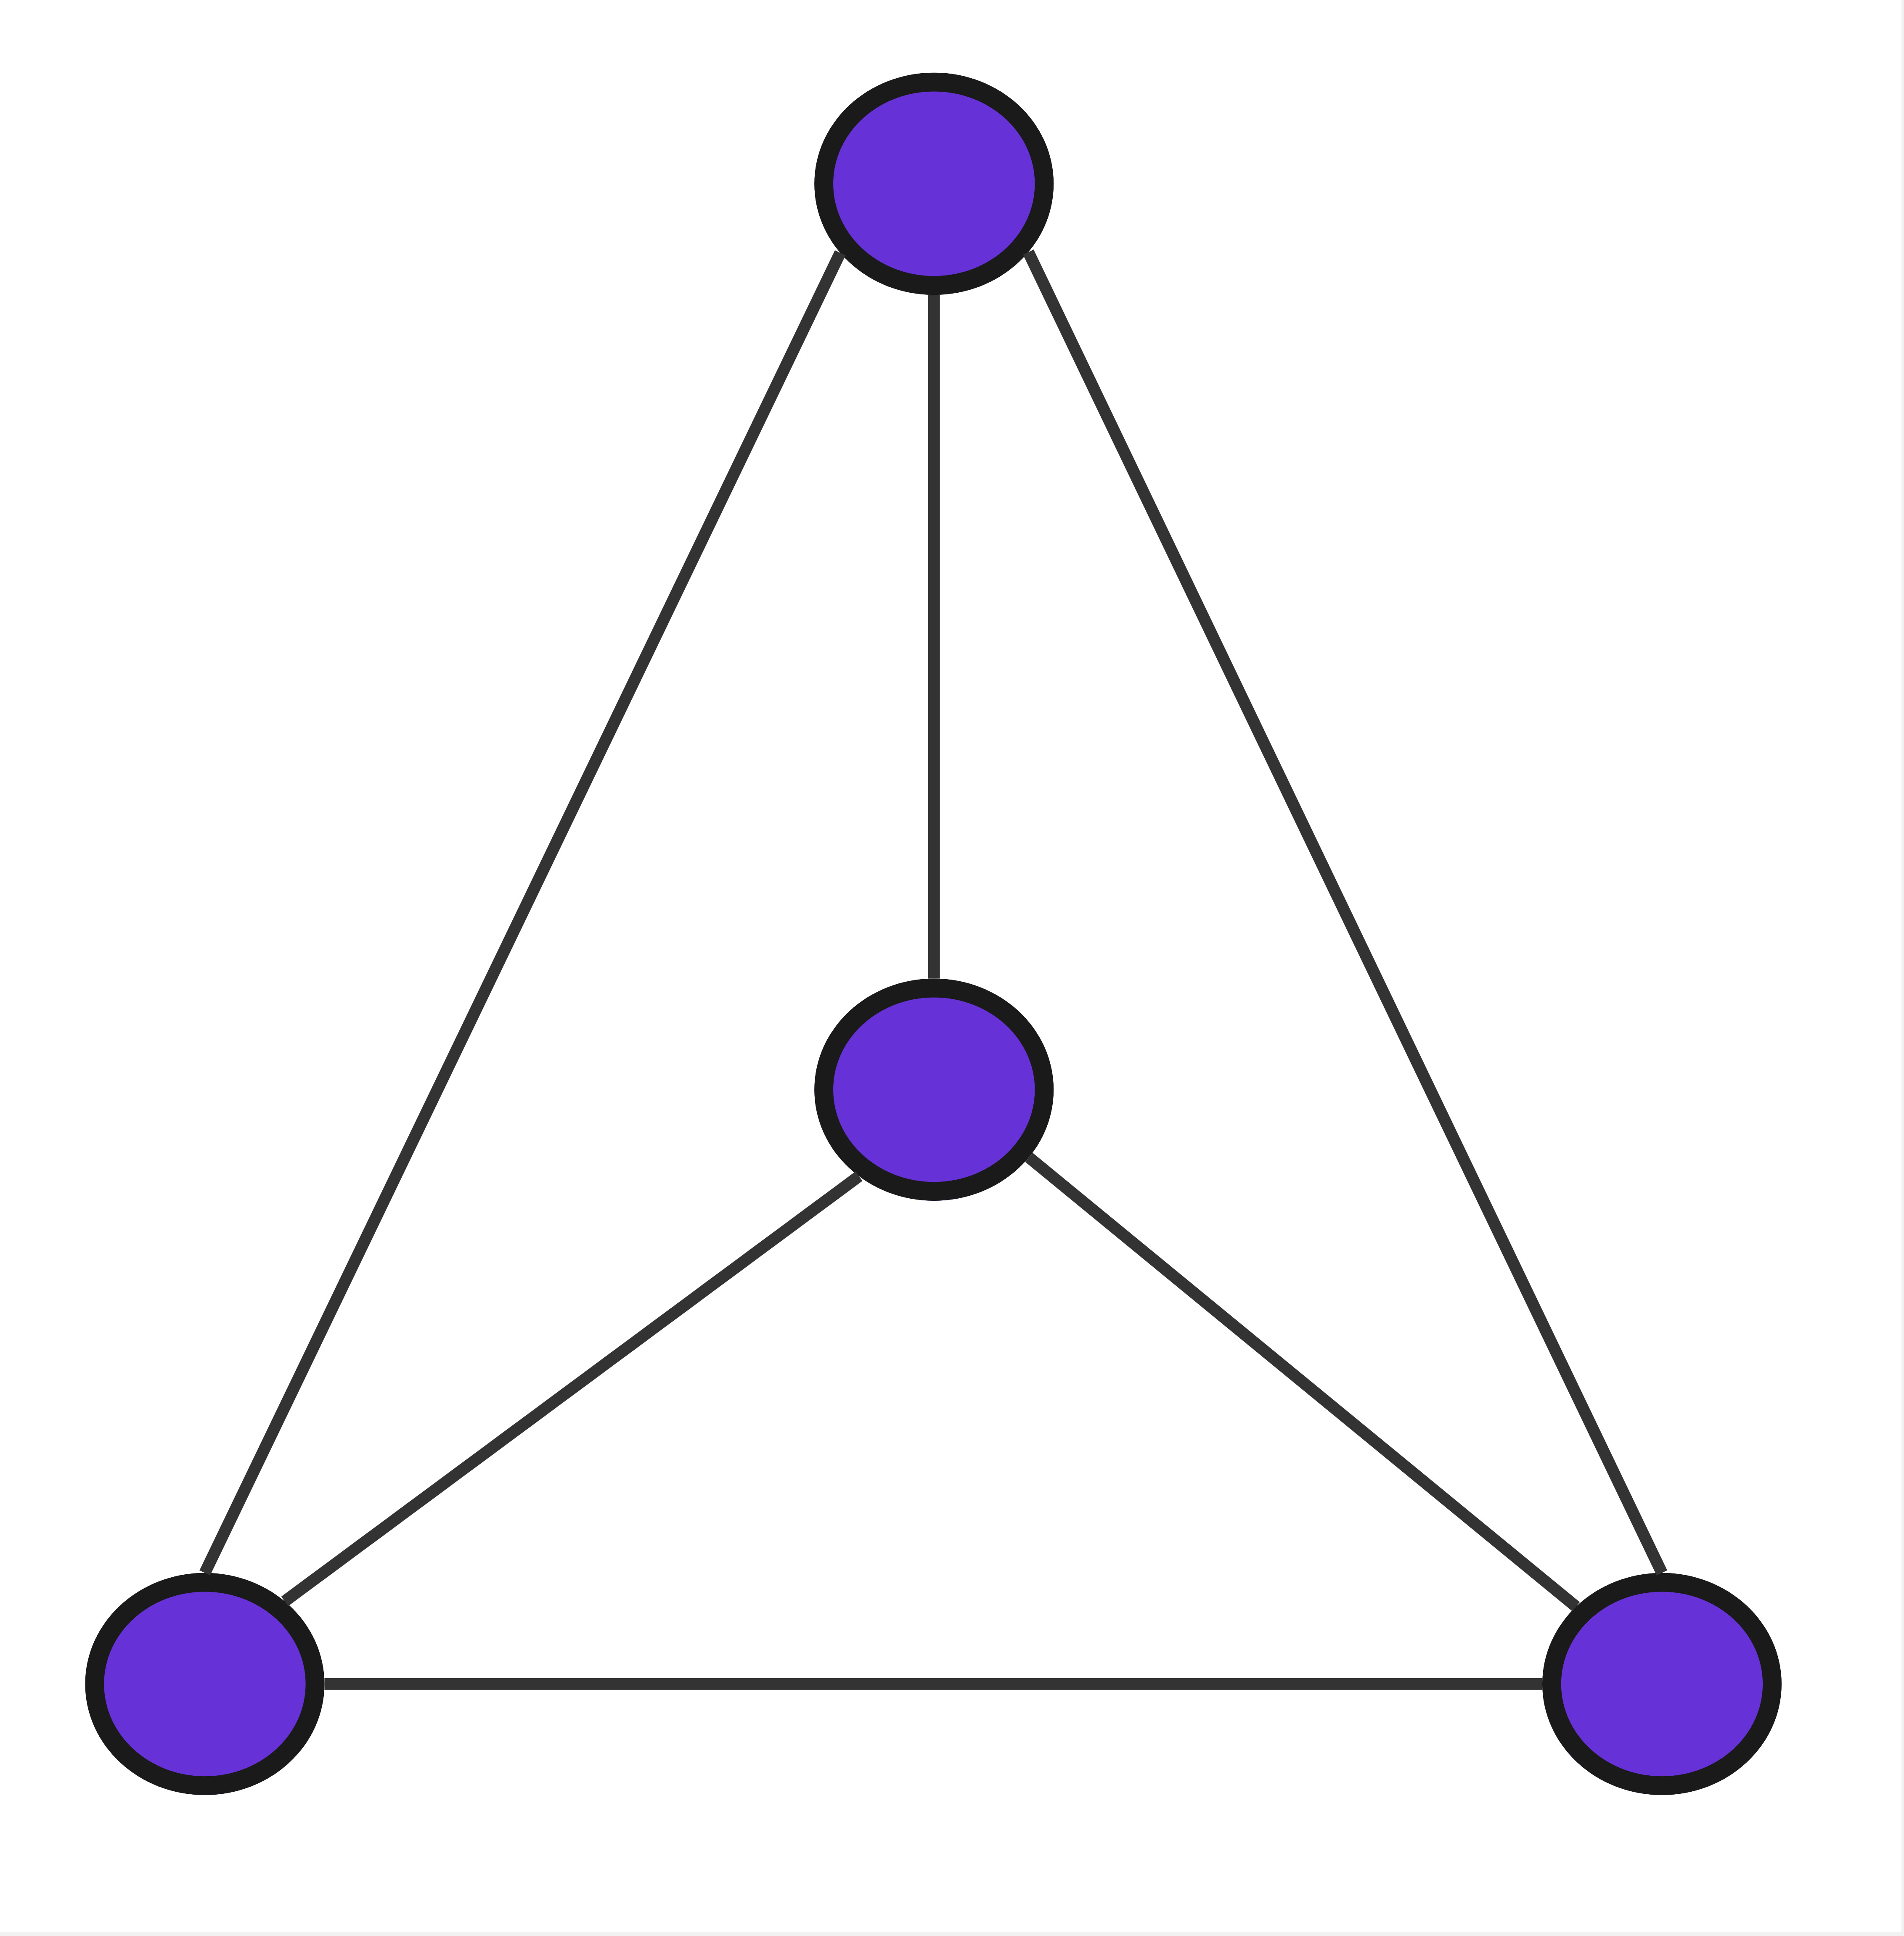
\includegraphics[width=0.9\linewidth]{images/k4_graph.jpg}
            \caption*{\textit{$K_4$}}
        \end{figure}
    \end{columns}
\end{frame}

\begin{frame}{Quiz}
  \centering
  \Large
  Qual dos três grafos a seguir é planar?
  \bigbreak
  \begin{minipage}{\linewidth}
    \centering
    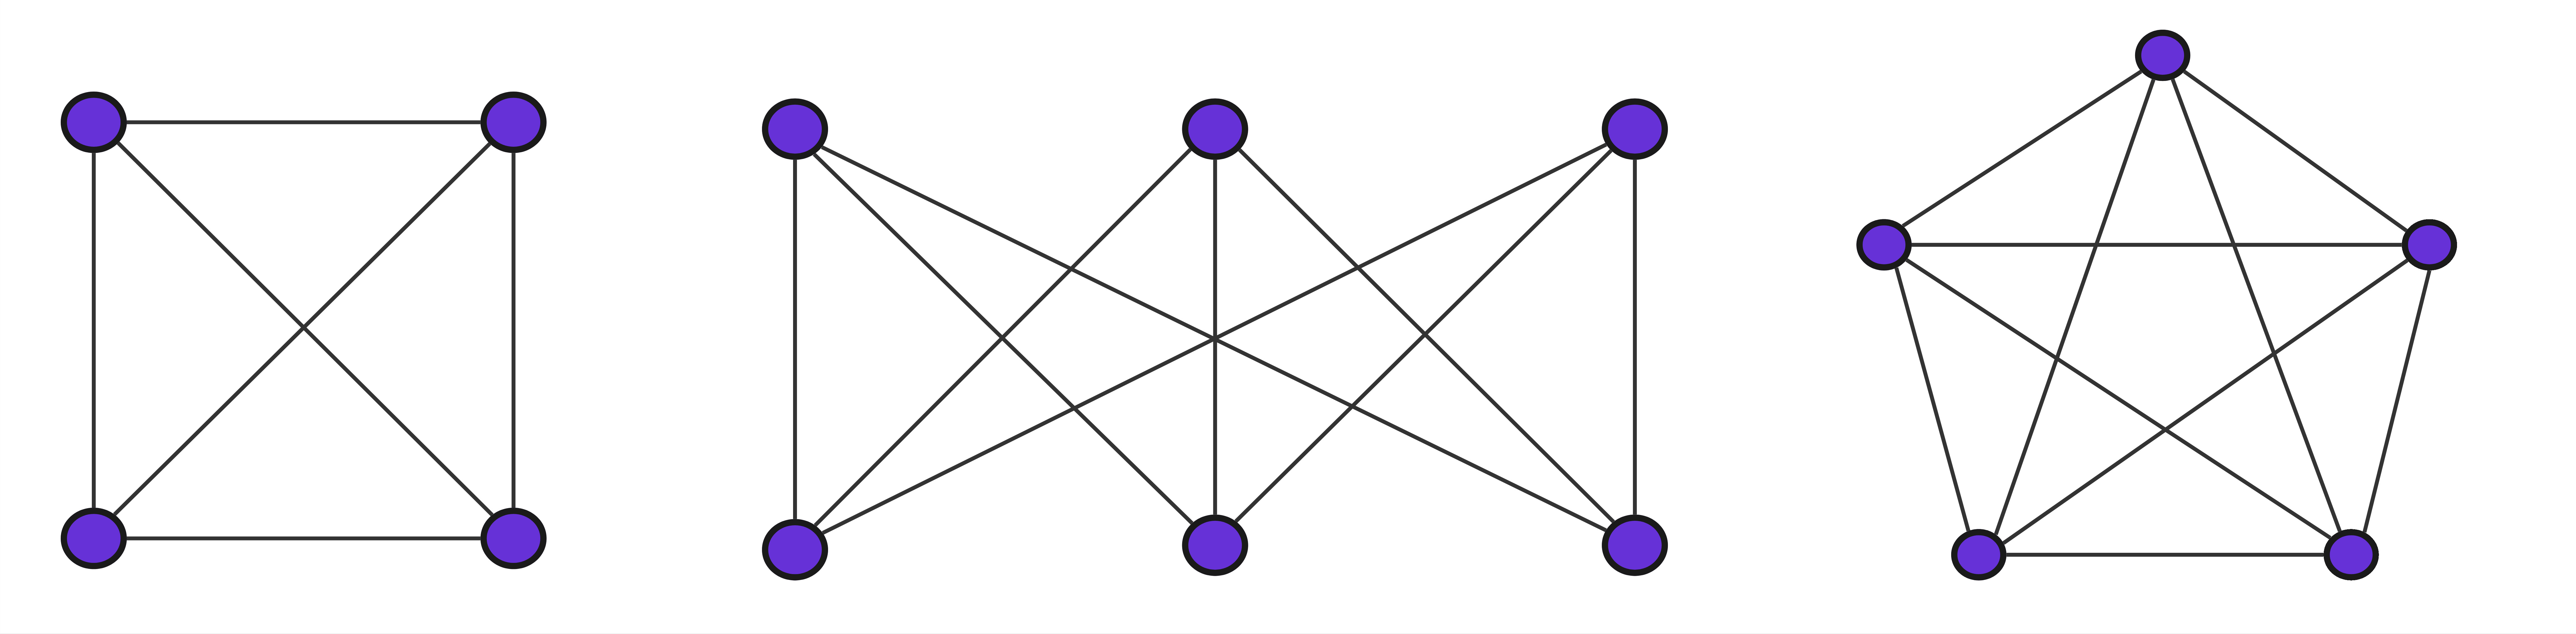
\includegraphics[height=2.5cm]{images/quiz_1.jpg}
  \end{minipage}
\end{frame}

\begin{frame}{Quiz}
  \centering
  \Large
  Qual dos três grafos a seguir é planar?
  \bigbreak
  \begin{minipage}{\linewidth}
    \centering
    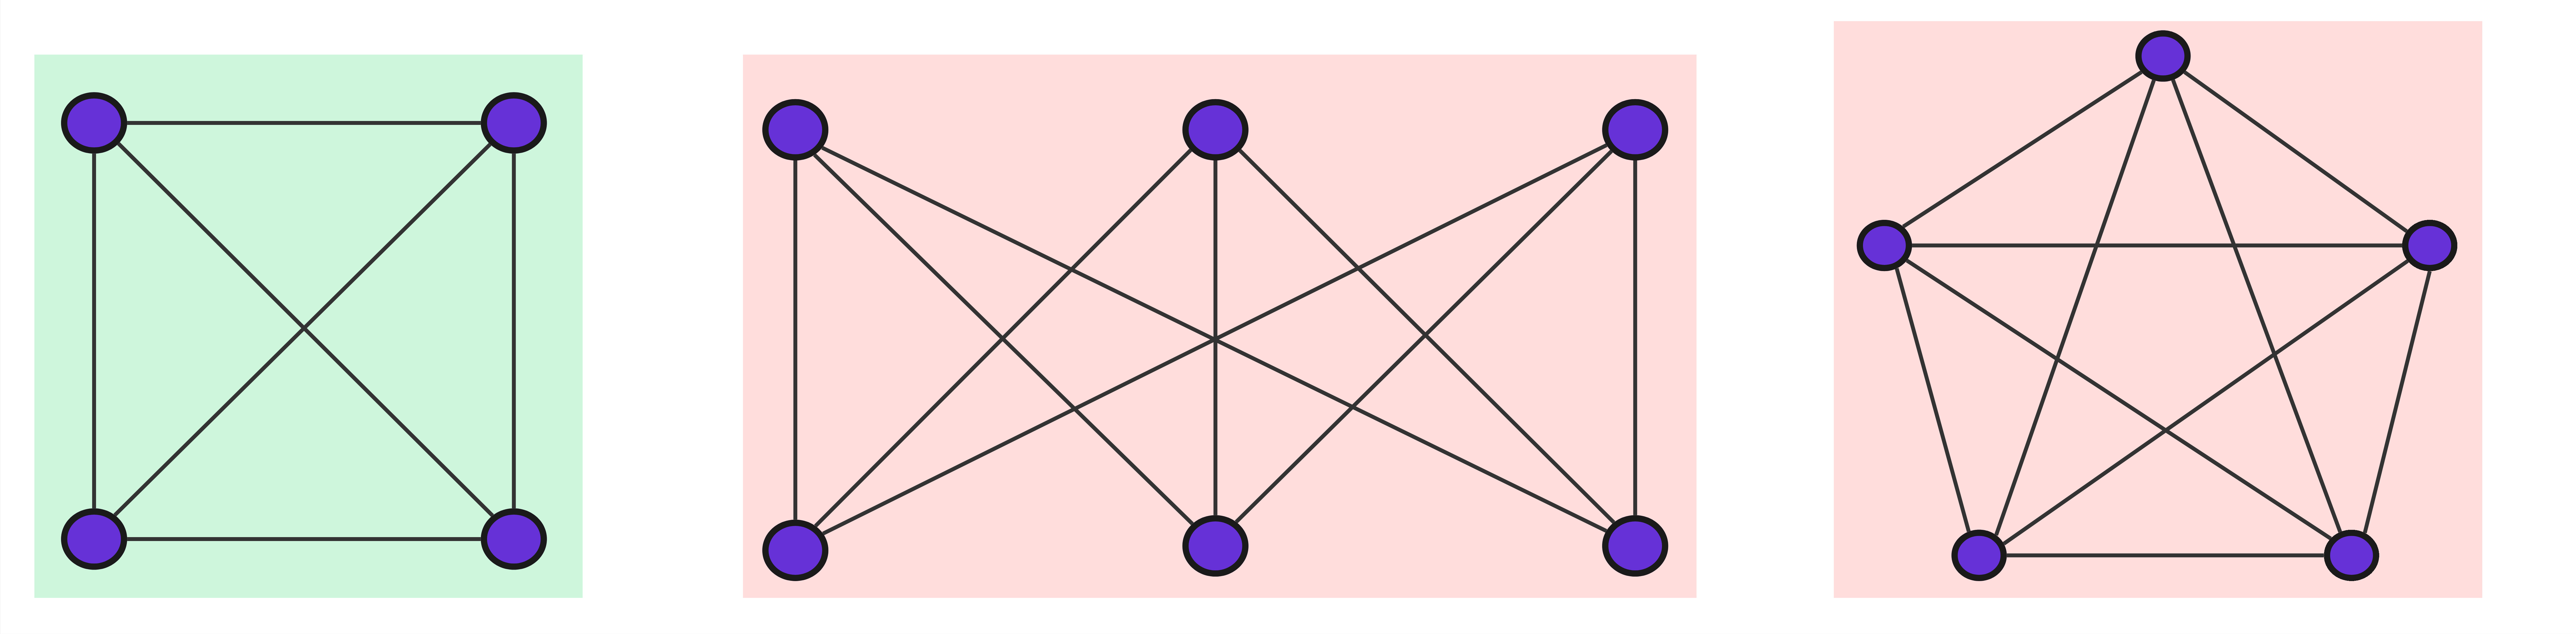
\includegraphics[height=2.5cm]{images/quiz_1_solved.jpg}
  \end{minipage}
\end{frame}

\begin{frame}{Mais Definições}
    \begin{minipage}{\linewidth}
        \centering
        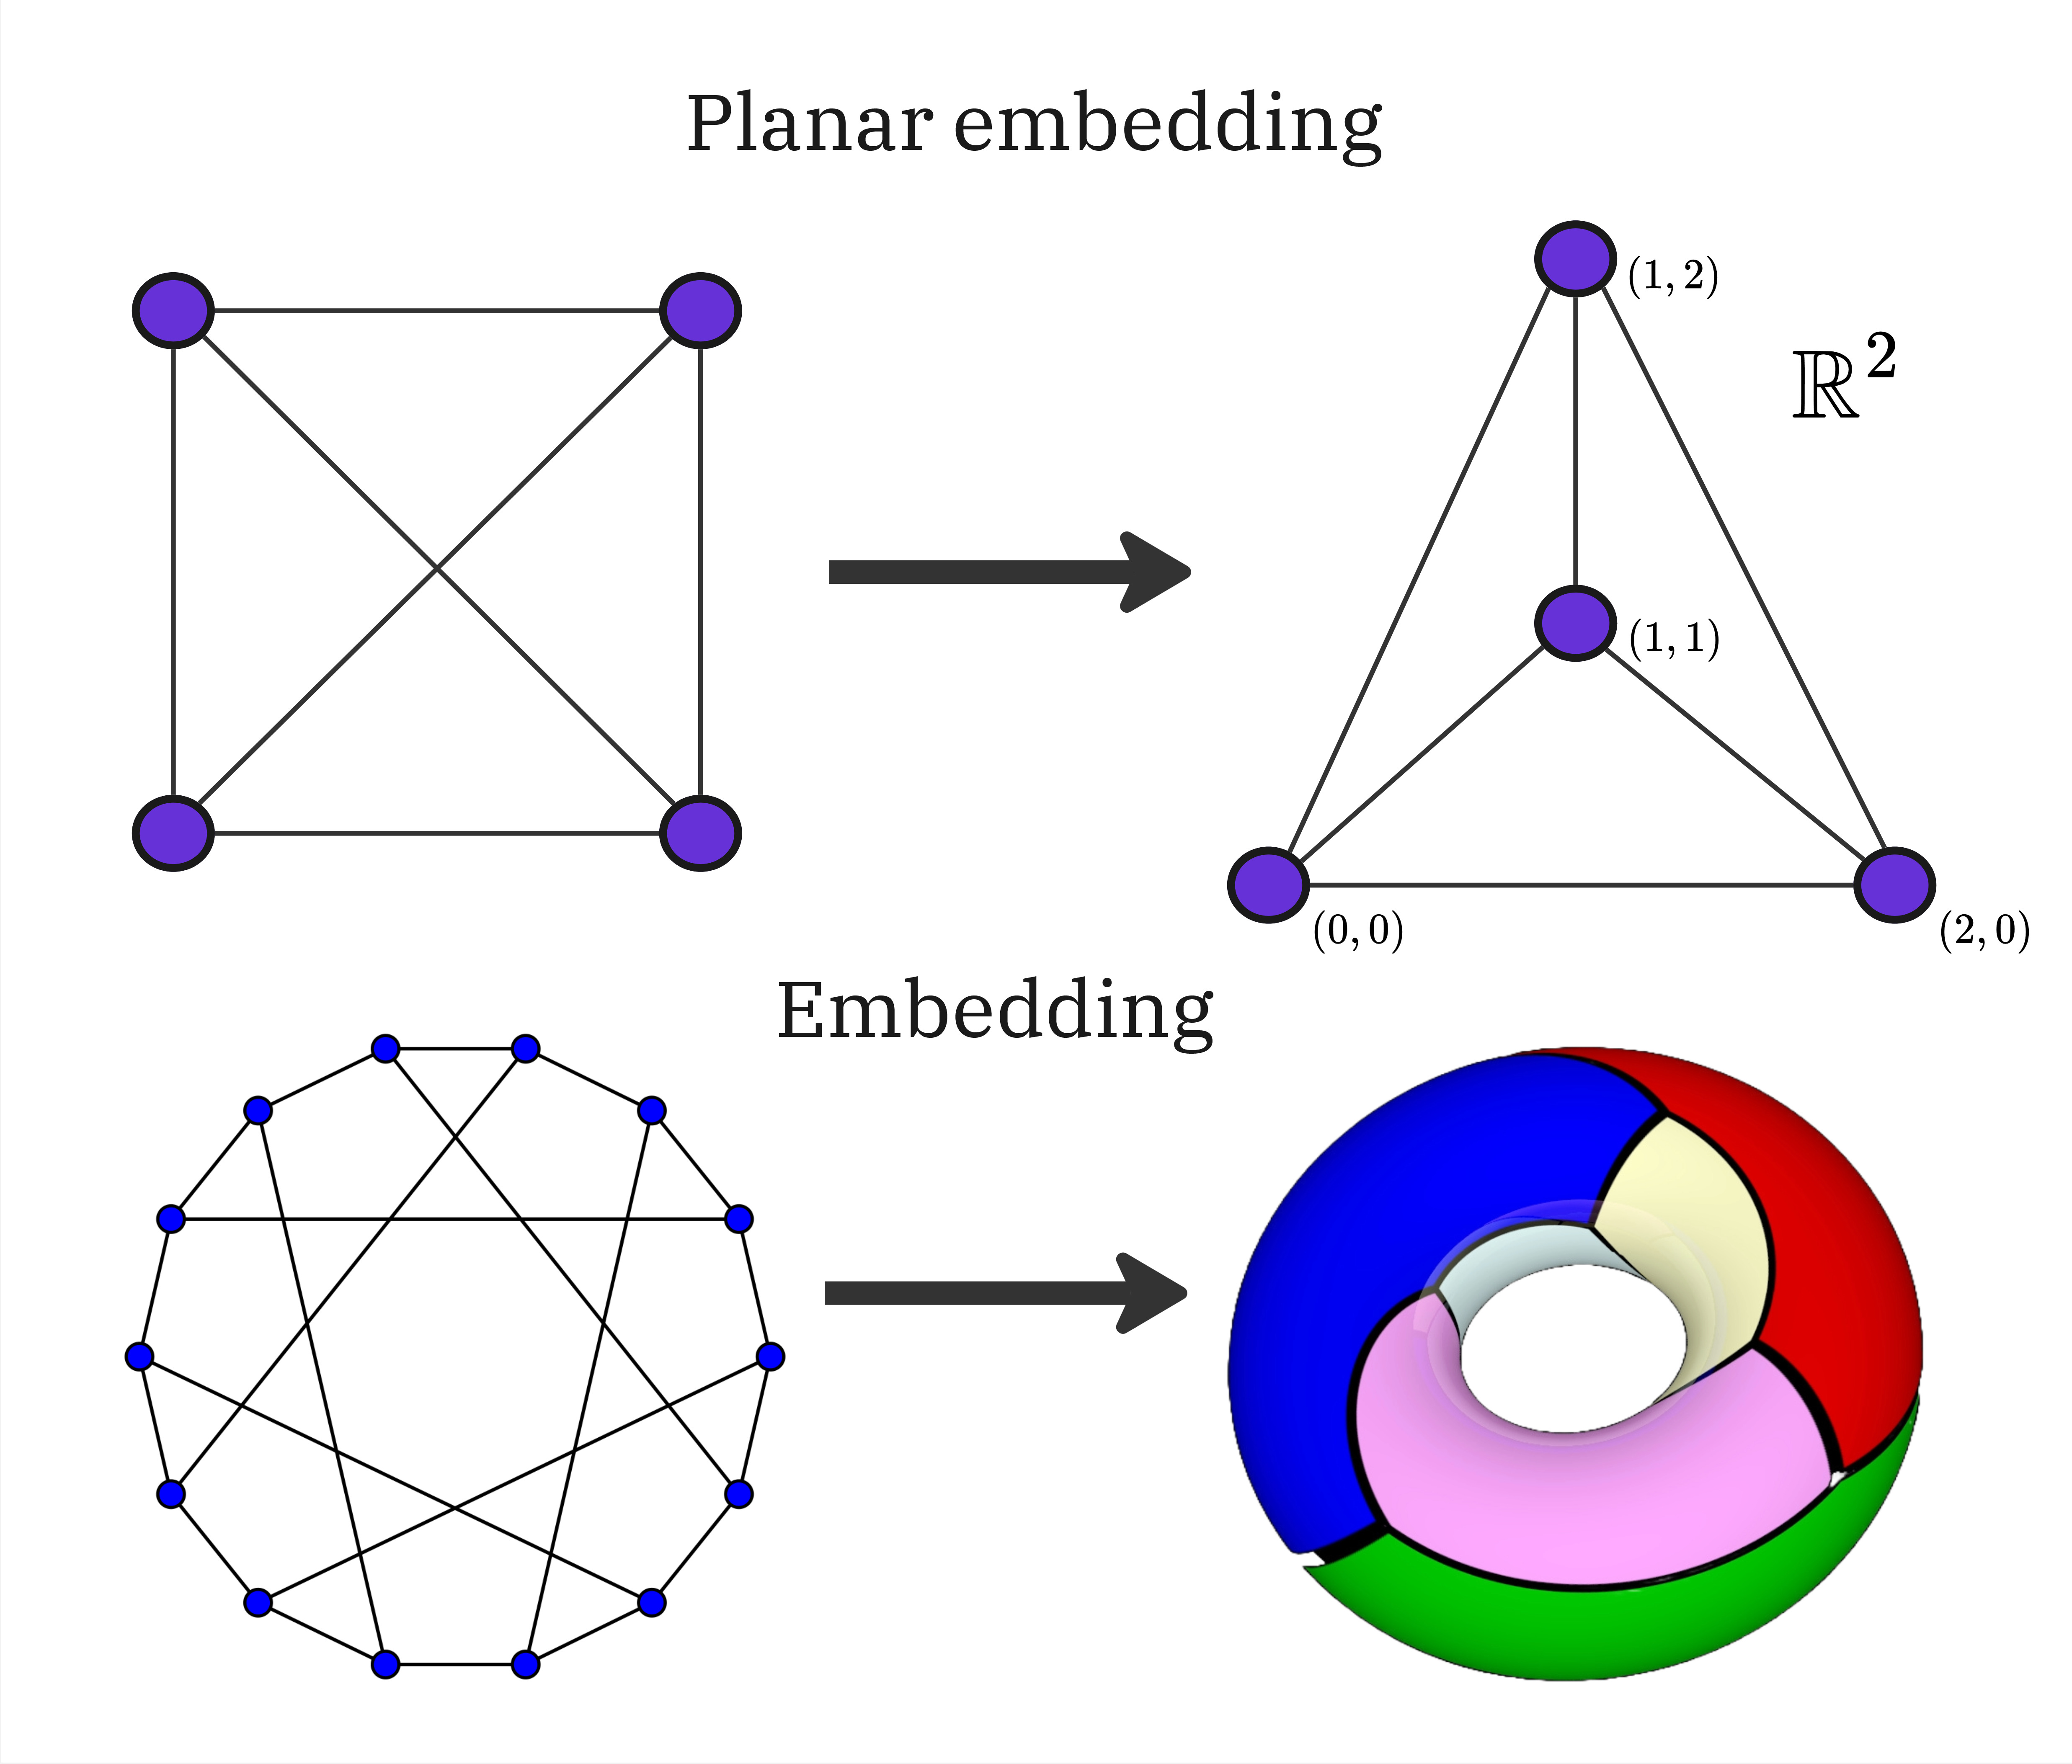
\includegraphics[height=8cm]{images/embedding.jpg}
    \end{minipage}
\end{frame}

\begin{frame}{Muito Mais Definições}
    \centering
    \large
    Um grafo é \textbf{\emph{outerplanar}} se admite uma imersão planar com todos os vértices na face externa.
    \bigbreak
    \begin{minipage}{\linewidth}
        \centering
        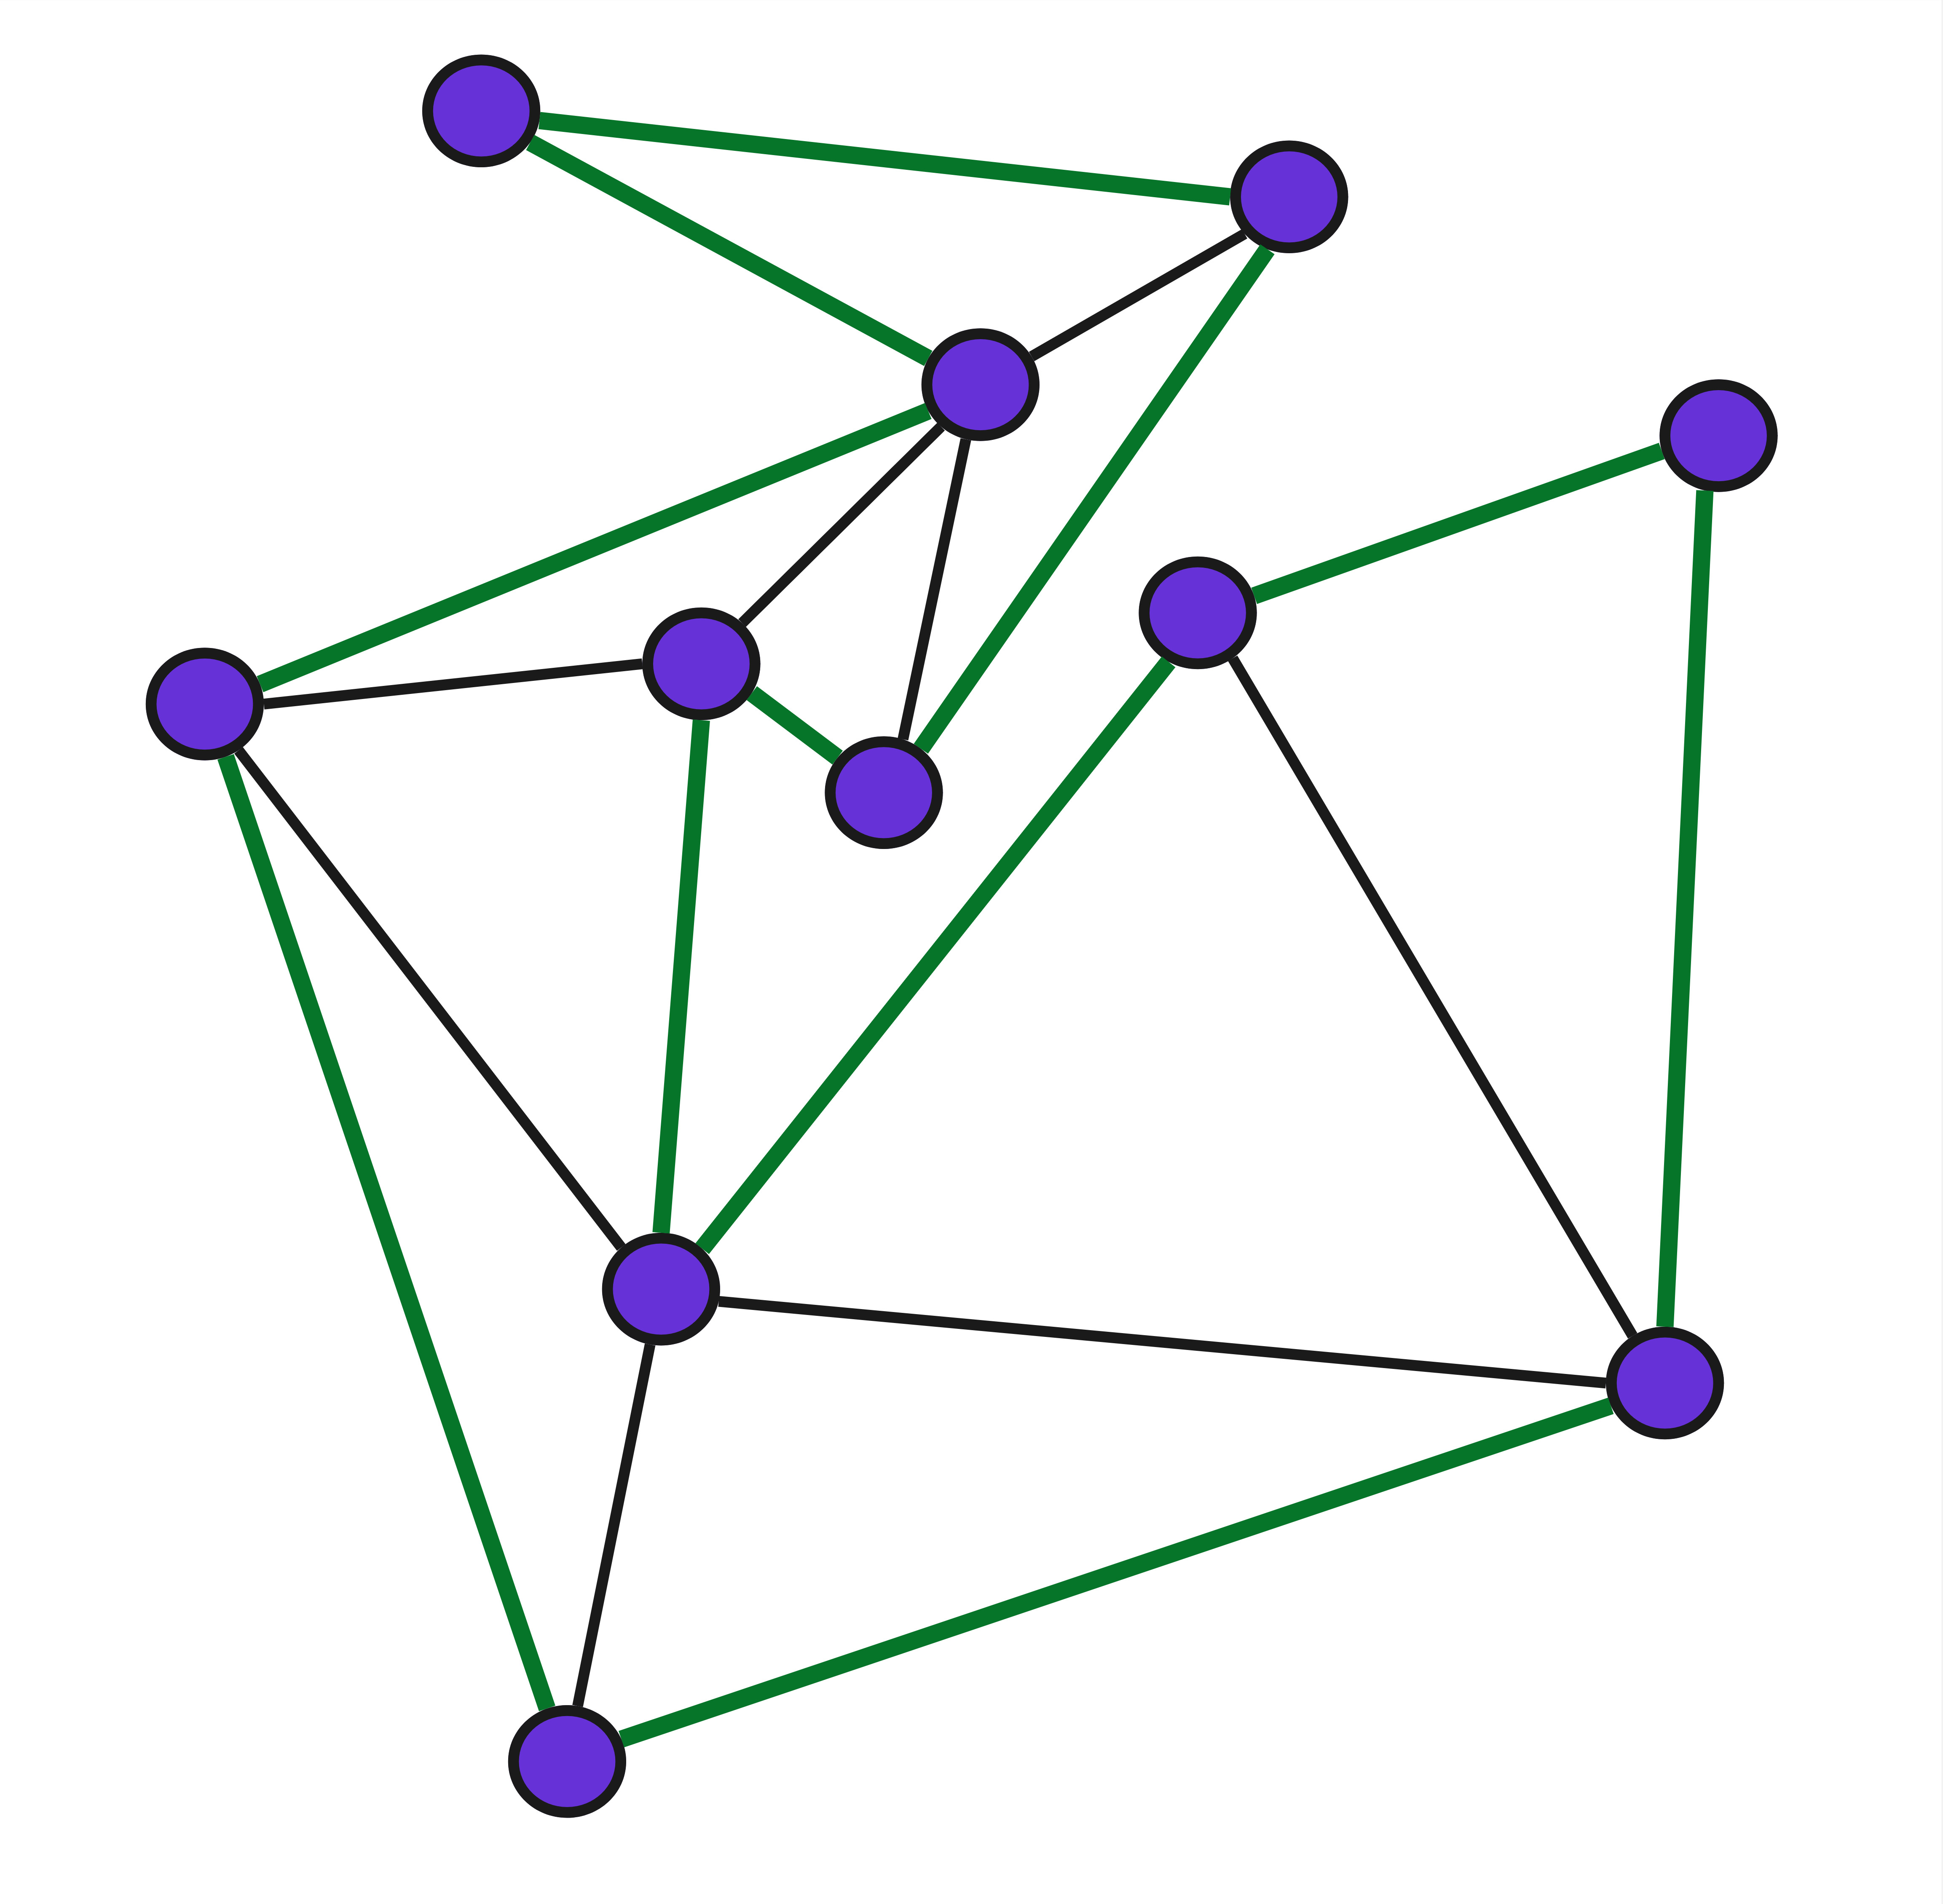
\includegraphics[height=3cm]{images/outerplanar.jpg}
    \end{minipage}
    \pause\bigbreak
    Todo grafo planar é outerplanar?\\
    \pause
    Não! Considere o $K_4$
    \bigbreak
    \begin{minipage}{\linewidth}
        \centering
        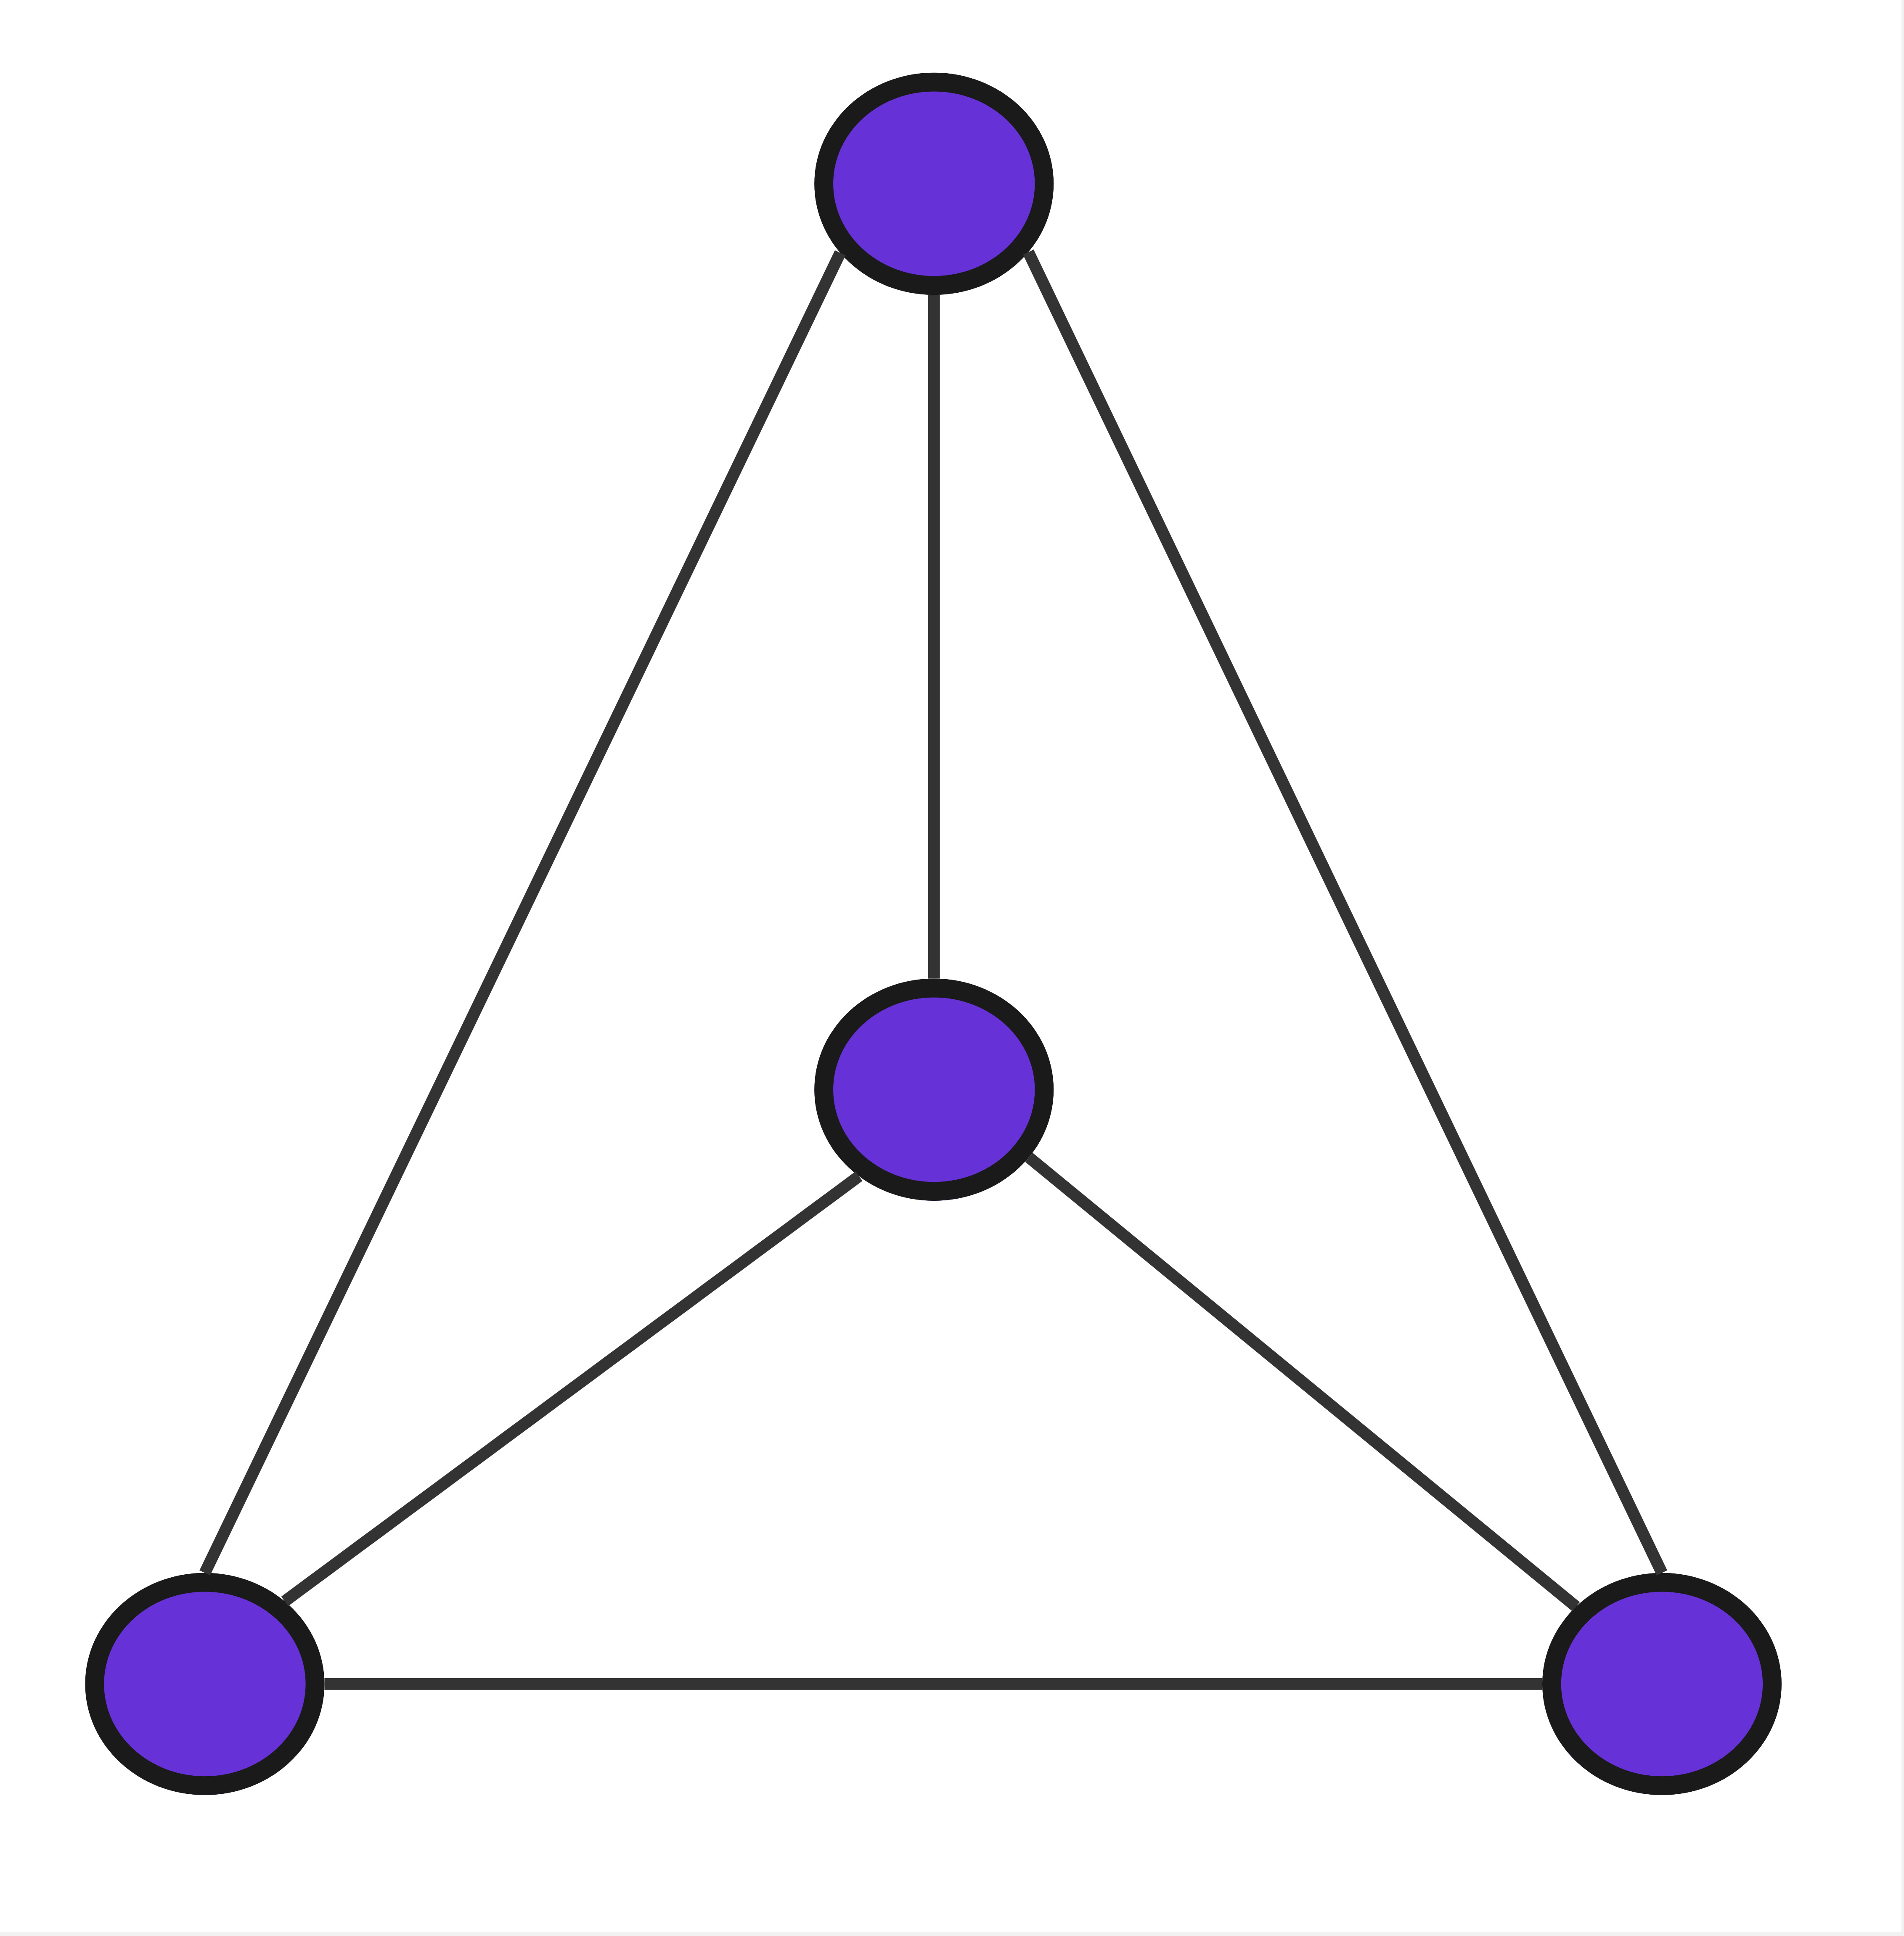
\includegraphics[height=2cm]{images/k4_graph.jpg}
    \end{minipage}
\end{frame}

\begin{frame}{Ainda Mais Definições}
    \centering
    \LARGE
    Nível 1
    \bigbreak
    \begin{minipage}{\linewidth}
        \centering
        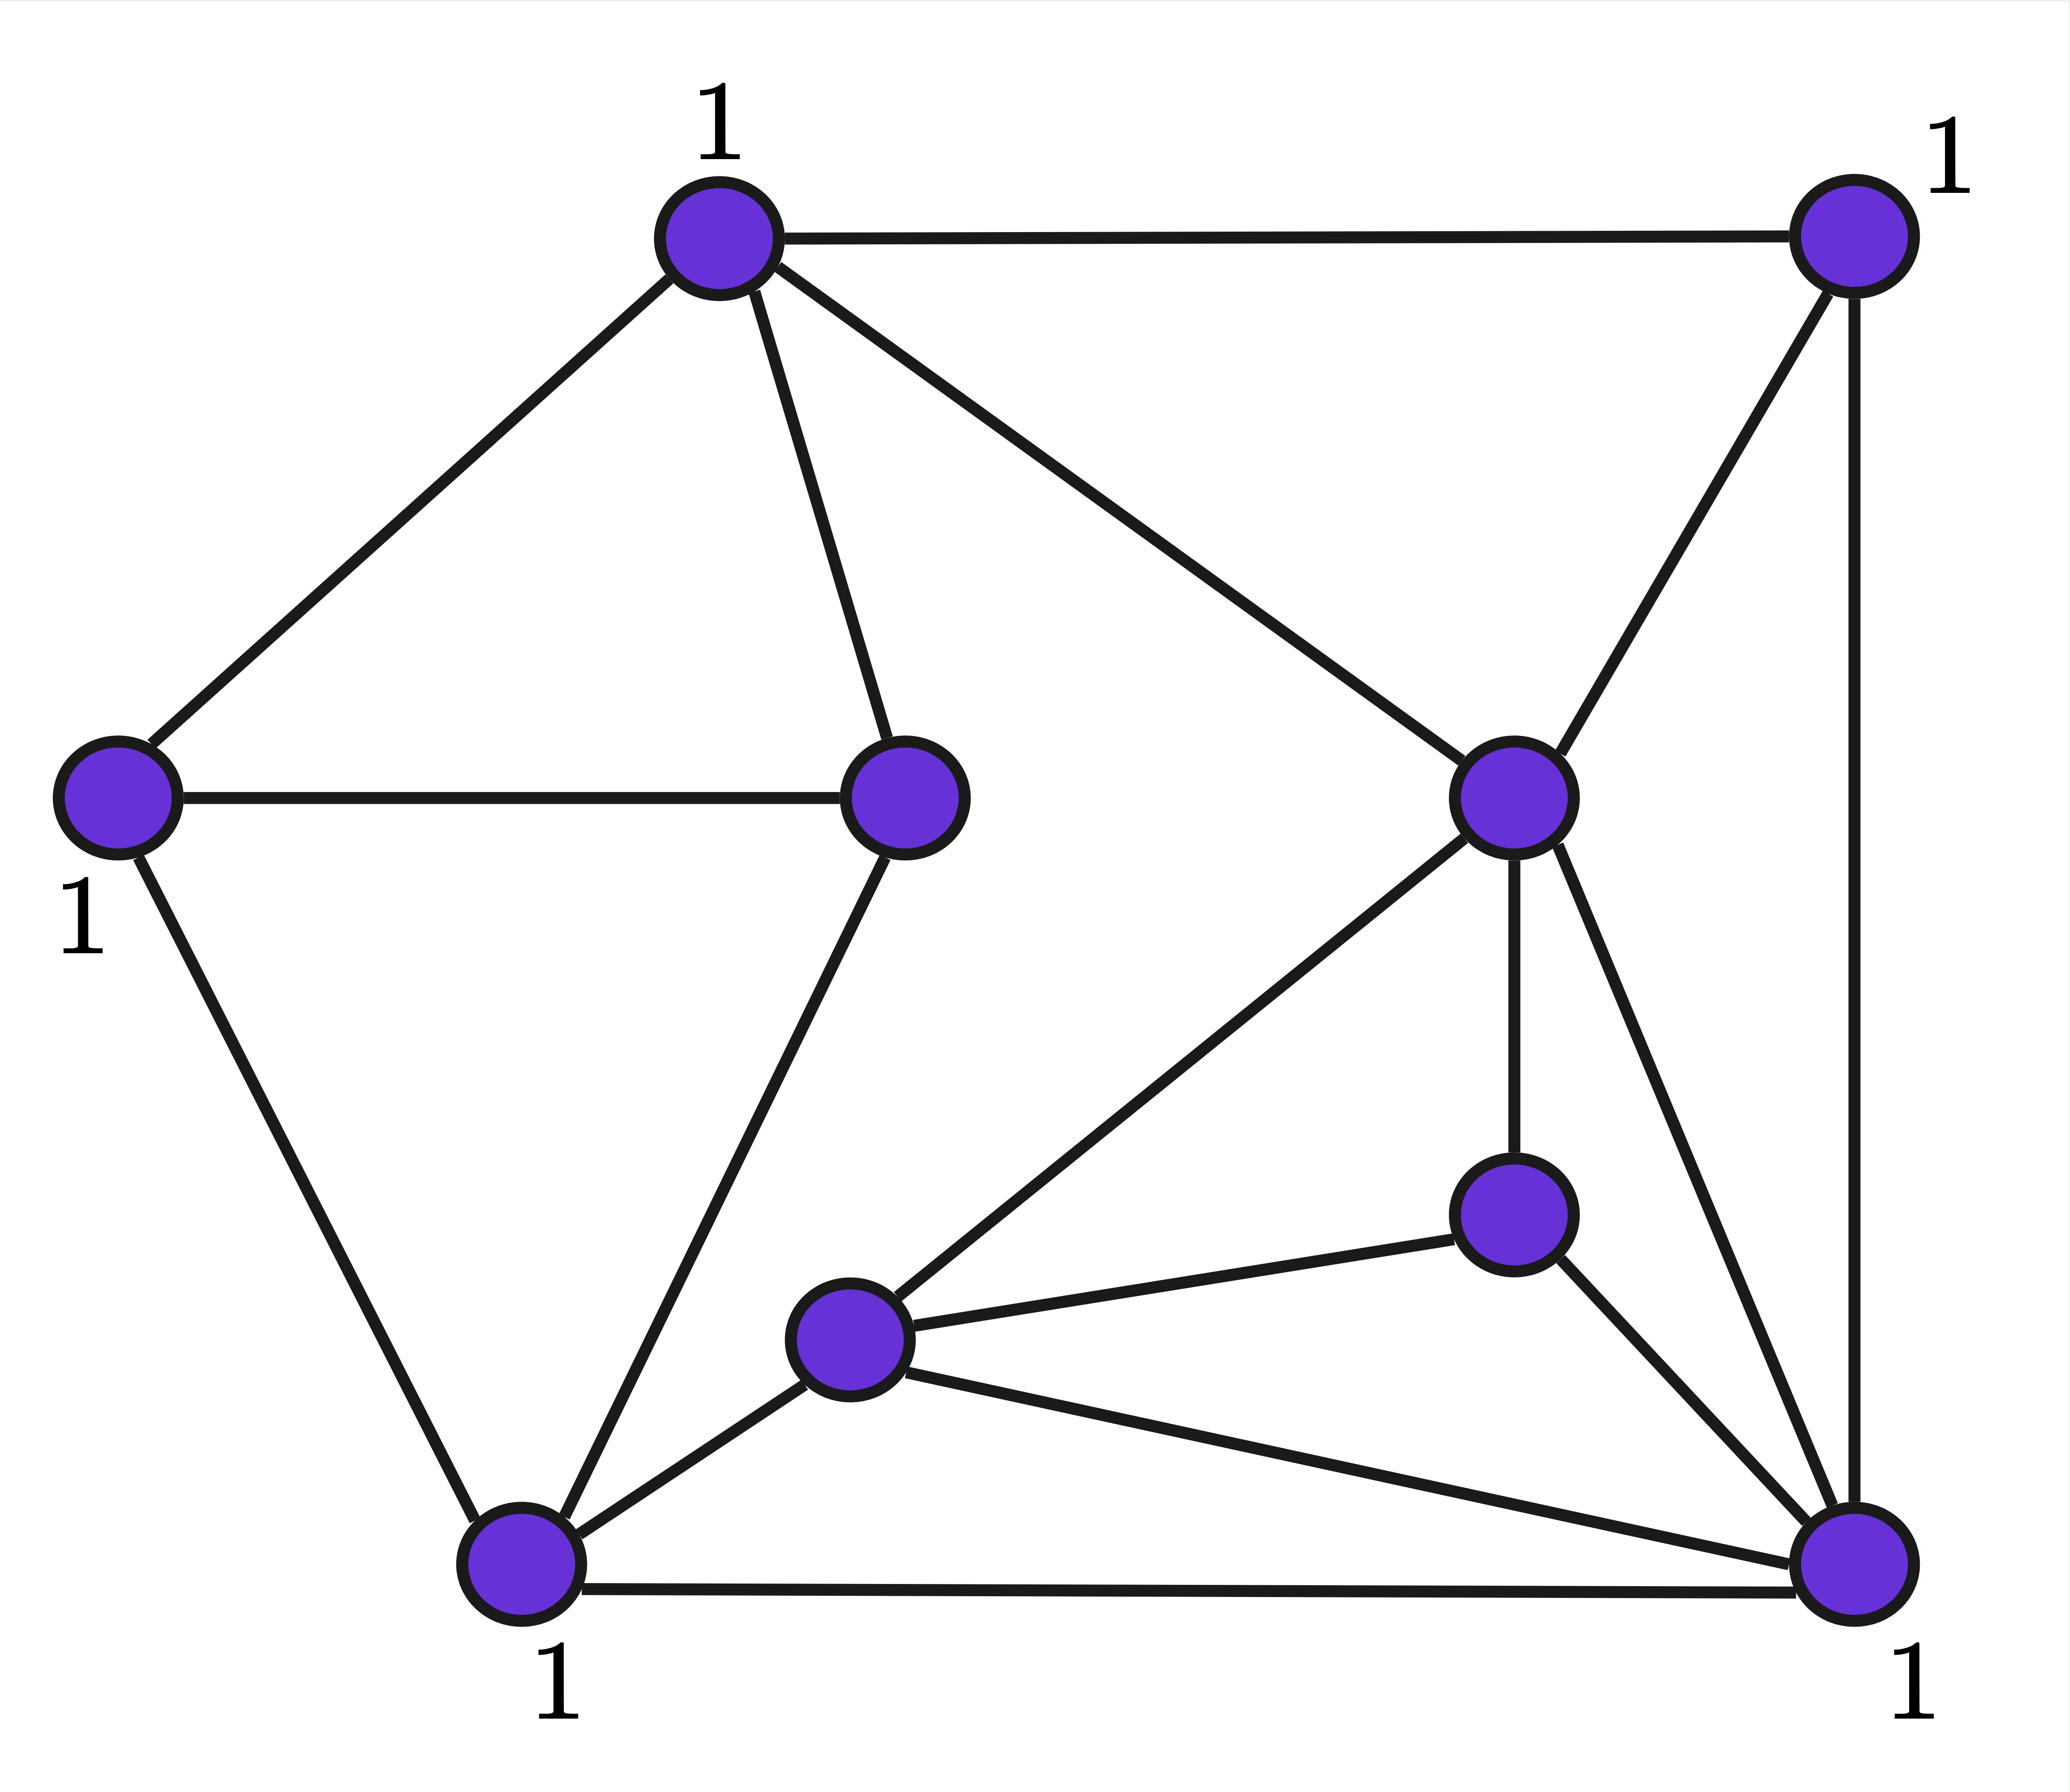
\includegraphics[height=5cm]{images/k_outerplanar_1.jpg}
    \end{minipage}
\end{frame}

\begin{frame}{Ainda Mais Definições}
    \centering
    \LARGE
    Nível 1 e Nível 2
    \begin{minipage}{\linewidth}
        \centering
        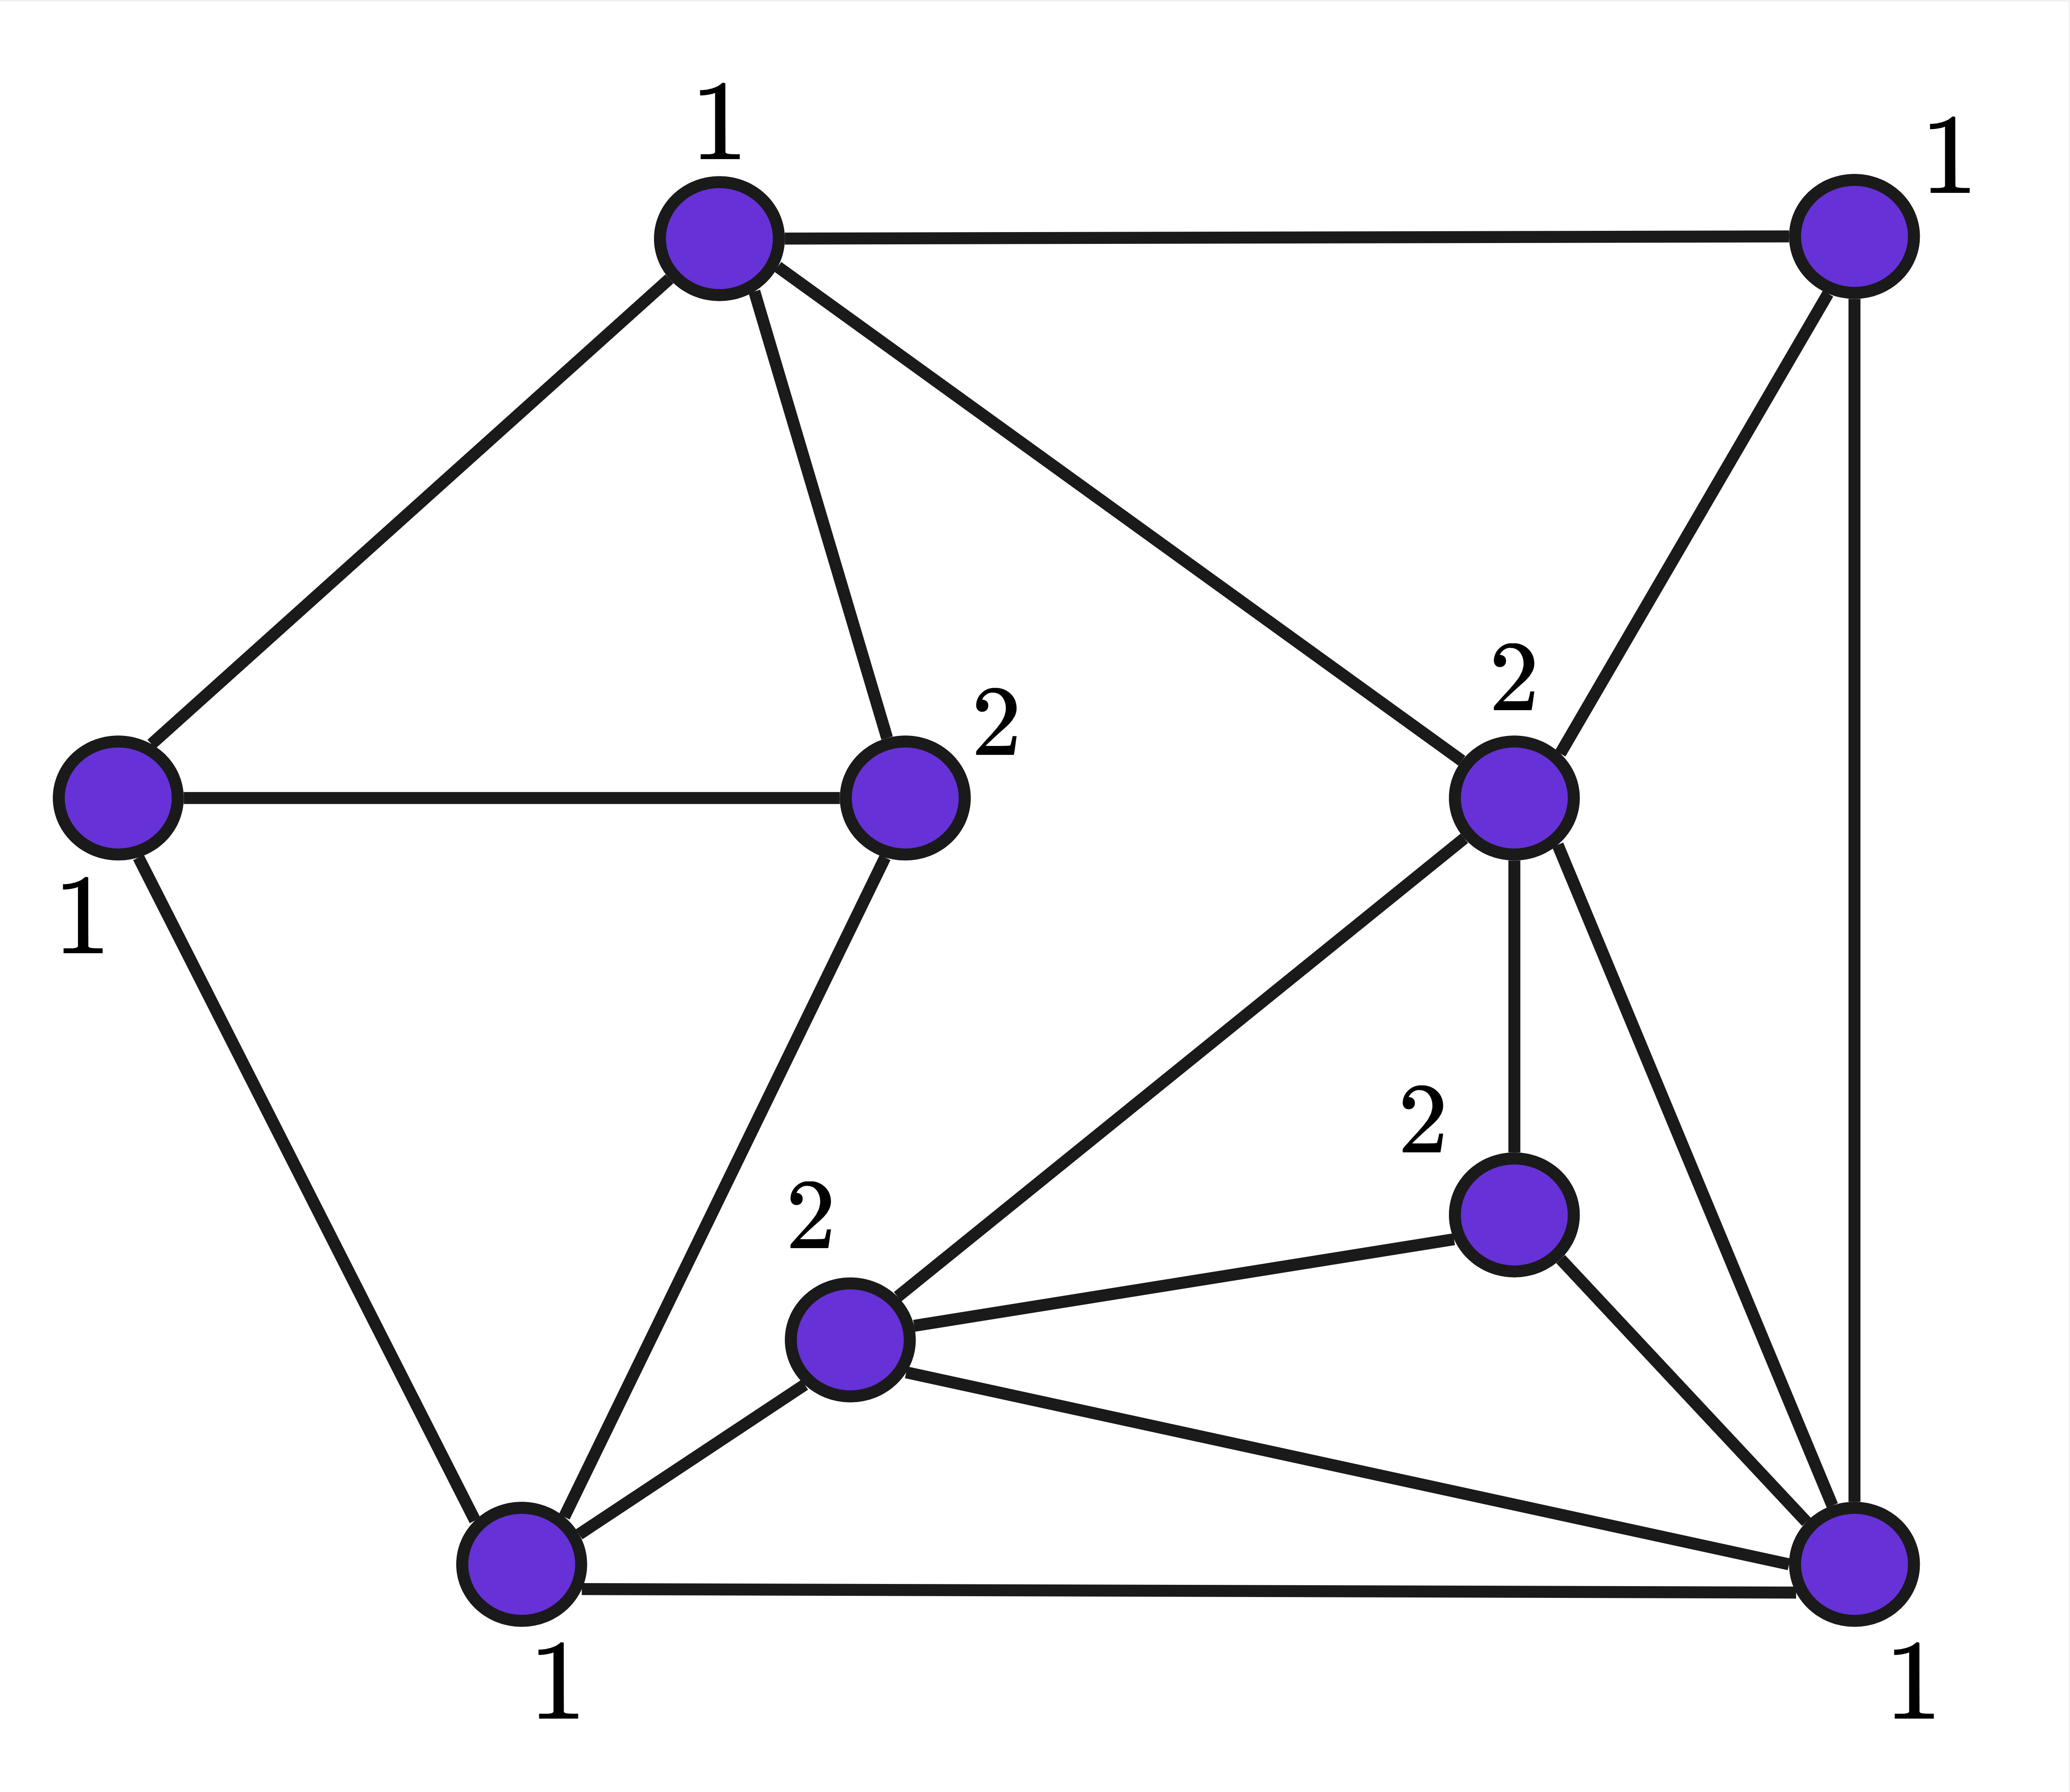
\includegraphics[height=5cm]{images/k_outerplanar_2.jpg}
    \end{minipage}
\end{frame}

\begin{frame}{Ainda Mais Definições}
    \centering
    \LARGE
    Nível 1, Nível 2 e Nível 3
    \begin{minipage}{\linewidth}
        \centering
        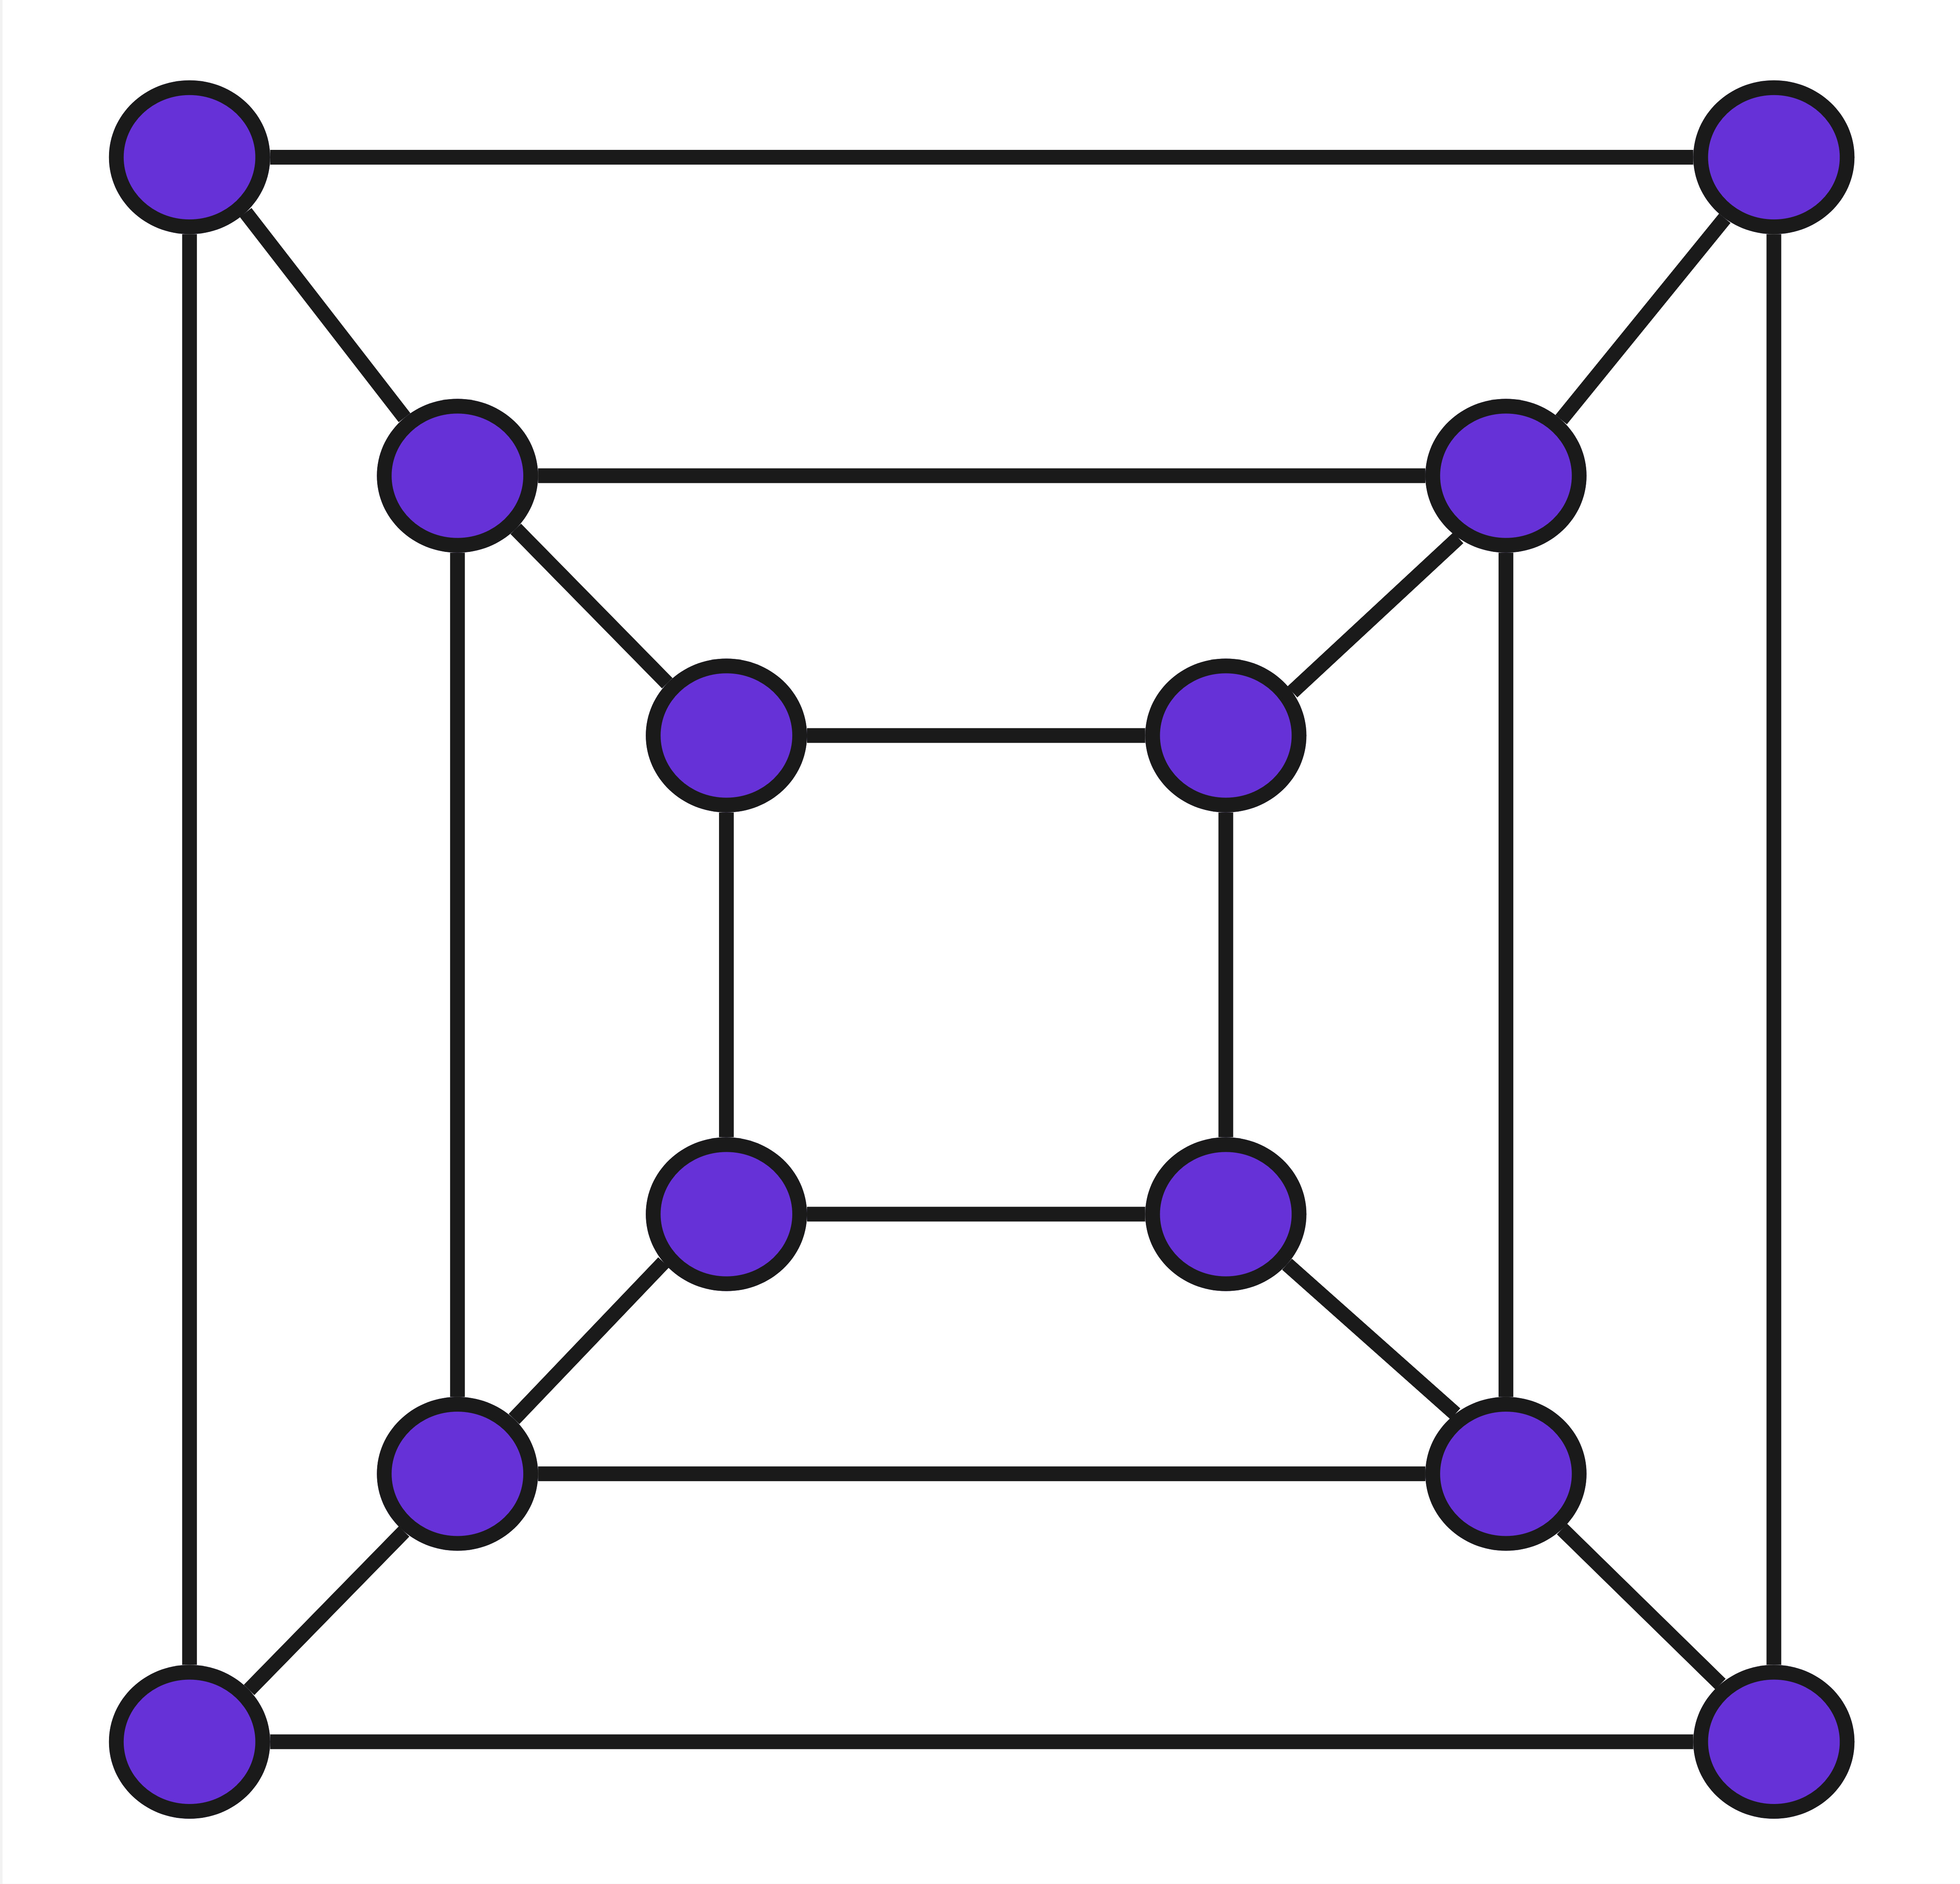
\includegraphics[height=5cm]{images/k_outerplanar_3.jpg}
    \end{minipage}
\end{frame}

\begin{frame}{Quando as Definições Vão Acabar!?}
    \begin{block}{Observação}
        Os vértices de nível $i$ de uma imersão planar de $G$ são aqueles que estão na face externa após a remoção dos vértices de níveis $1, \dots, i-1$ e suas arestas incidentes.
    \end{block}
    \bigbreak
    \begin{block}{Definição}
        Um grafo $G$ é \textbf{\emph{$k$-outerplanar}} se admite uma imersão planar na qual todos os seus vértices pertencem a níveis de $1$ até $k$.
    \end{block}
\end{frame}
